\chapter{Cause specific mortality rates: alcohol dependence}
\label{applications-csmr}

A key assumption of the GBD 2010 study is that there is only one cause leading to death categorical distribution of deaths.

similar to cannabis dependence \pageref{tab:app-substance_dependence}



\ref{theory-csmr}

Parkinson's disease \ref{intro-complete_ex}

cirrhosis \ref{applications-efx_country_level}, diarrhea \ref{applications-short_dur}, transport injury \ref{applications-double_dismod}

PF assumes that deaths with the condition are deaths caused by the condition.

\begin{equation}
TK.    
\end{equation}

This method implicitly separates $h_{f'}$ and $h_{f''}$ but does not try to explicitly represent both

    \begin{figure}[h]
        \begin{center}
            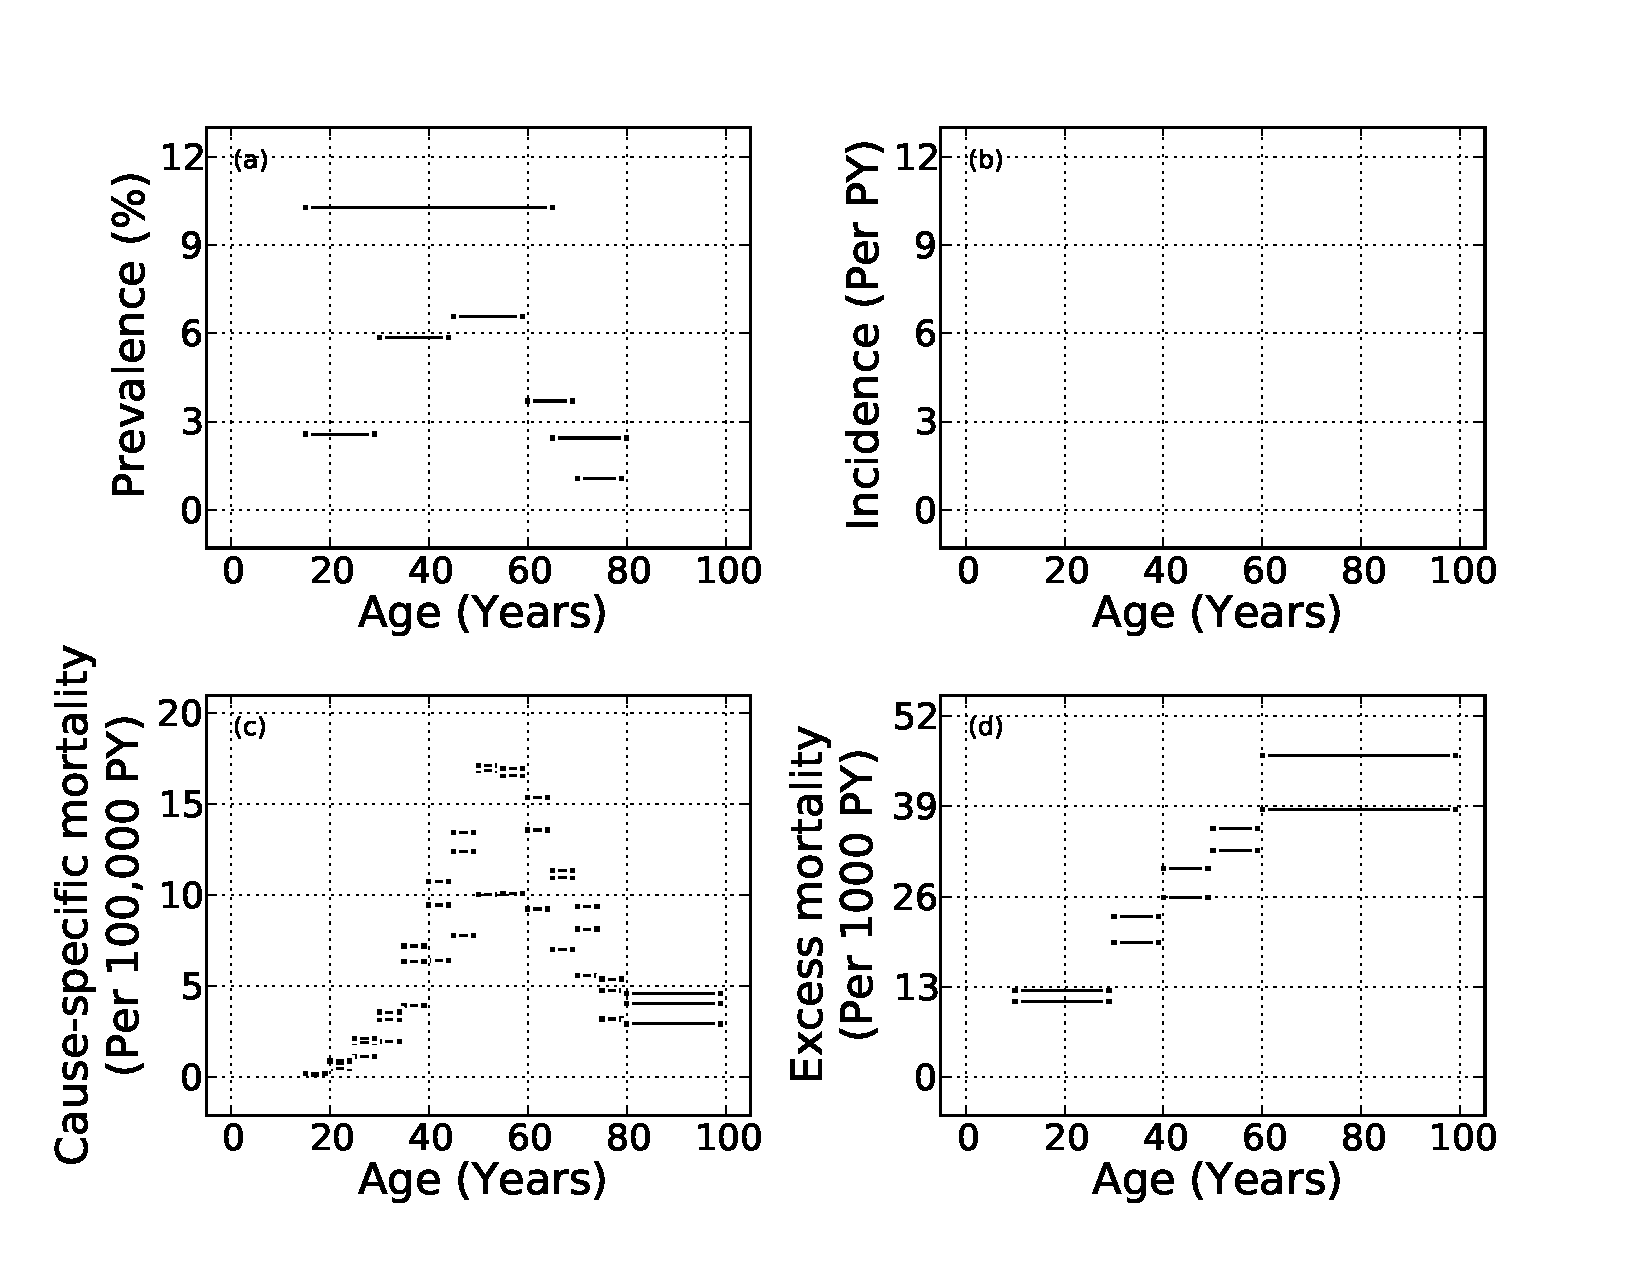
\includegraphics[width=\textwidth]{alcohol-data.pdf}
            \caption{Prevalence (panel (a)), incidence (panel (b)), cause-specific mortality (panel (c)) and excess mortality (panel (d)) of alcohol dependence in Western European males in 2005.}
            \label{fig:app-alcohol data}
        \end{center}
    \end{figure} 
    
    \begin{figure}[h]
        \begin{center}
            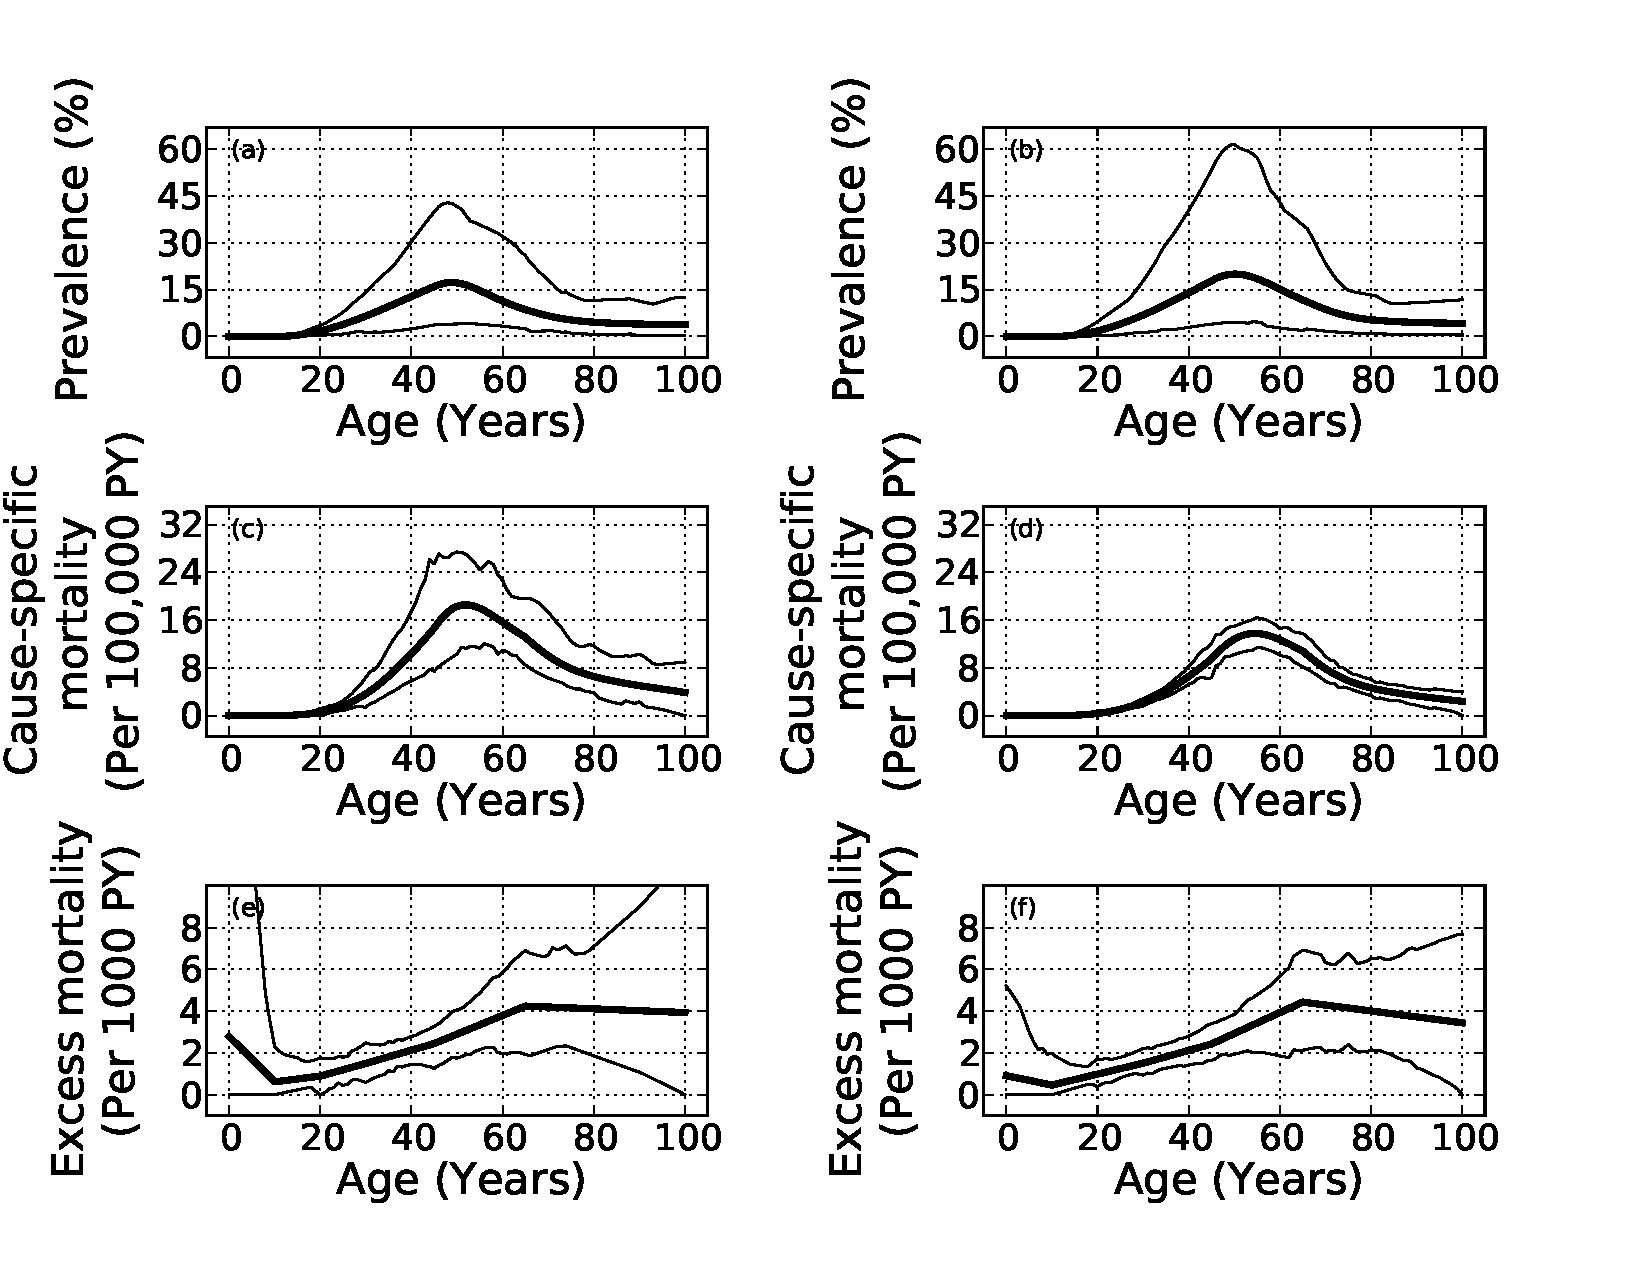
\includegraphics[width=\textwidth]{alcohol-csmr_v_pf.pdf}
            \caption{Prevalence (panel (a)), cause-specific mortality (panel (b)) and excess mortality (panel (d)) of alcohol dependence in Western European males in 2005.}
            \label{fig:app-alcohol compare}
        \end{center}
    \end{figure} 
